\scanpage{87}

\uline{\unsure{Schatten} norm} $N(x_1,-x_n)$ \uline{satisfies \deleted{\unsure{the|the}}\inserted{\deleted{of} the} condition considered} \uline{in the statement of \deleted{corollary 1}}\inserted{Theorem 1, 2°} \deleted{\unsure{recalled above}}\inserted{for the function $f$. We conclude from this,} if $(\rho_i)$ \deleted{$\unsure{\rho(\sigma_i|\rho(x)}$} and $(\sigma_i)$ are as in the theorem :

\reversemarginpar
\margin{\textcircled{\unsure{11|13}} $N(\rho_1,-\rho_n)\leq N(\sigma_1,-\sigma_n)$ and more generally, taking into account a preceding remark, and \deleted{\unsure{so that}} setting for $1\leq k\leq n$ : $N(\rho_1,-\rho_k)=N(\rho_1,-\rho_k,0-0)$ \textcircled{12} $N(\rho_1,-\rho_k)\leq N(\sigma_1,-\sigma_k)$ for $1\leq k\leq n$}
\normalmarginpar

\deleted{From =, \unsure{if we know} that the function $(e^{t_i})^p$ being a \unsure{convex function}} \deleted{\inserted{\uline{the function} $f(r_1,-r_n)=r_1^p\unsure{-|+}+r_n^p$,} \uline{$p$ is an arbitrary real number, satisfies the \deleted{\unsure{conditions}}} \uline{conditions} \deleted{\unsure{of the lemma}} \uline{considered in corollary 1}, \deleted{\unsure{therefore} \uline{under hypothesis b, and = \deleted{\unsure{all the}}\inserted{\unsure{we have|the|case a}} conditions considered} \uline{under hypothesis a.}}}

Consequently, \deleted{\unsure{under the condition,}}\inserted{under the conditions} of hypothesis b, \deleted{\unsure{we}} $(\prod_1^M\rho_i\leq\prod_1^M\sigma_i\ \inserted{\text{for }1\leq M\leq n},\ \prod_1\rho_i=\prod_1^n\sigma_i\ne0)$ we shall have

\[
\begin{array}{ll}
(\unsure{1|9}5) & \displaystyle\sum_1^n\rho_i^p\leq\sum_1^n\sigma_i^p\qquad(p\text{ real.})
\end{array}
\]

\deleted{\unsure{and in case a|and under the conditions}} \inserted{and if $p\geq0$,} we shall have, provided that $\prod_1^M\rho_i\leq\prod_1^M\sigma_i$ for \inserted{$1\leq M\leq n$}, \deleted{we shall have}

\[
\begin{array}{ll}
\deleted{\unsure{(12)}}\inserted{(16)} & \displaystyle\sum_1^k\rho_i^p\leq\sum_1^k\sigma_i^p\qquad(p\geq0,\ \deleted{\unsure{and}} k=1-n.)
\end{array}
\]

\deleted{Let us note moreover that 2 \inserted{\deleted{\unsure{positive}}} \inserted{positive} \unsure{systems|sequences} $(\rho_i),(\sigma_i)$ \unsure{given|forming}, \deleted{\unsure{as soon as}} satisfying the inequalities (16), for \deleted{every} $k$, and \deleted{every} $p$ \unsure{integer|real} $\geq0$, we can \uline{\unsure{property}} \unsure{converse|conversely}}

\deleted{\unsure{We can arrive at}}

\reversemarginpar\margin{\uline{Theorem 2}}\normalmarginpar
(\uline{First Convexity Theorem in Hilbert spaces})

\reversemarginpar
\margin{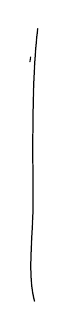
\begin{tikzpicture}[x=1cm,y=1cm]
\draw[line width=.45pt] (0,.02) .. controls (-.08,-.65) and (-.06,-1.5) .. (-.06,-2.3) .. controls (-.08,-2.8) and (-.12,-3.15) .. (-.04,-3.45);
\draw[line width=.4pt] (-.09,-.34)--(-.10,-.41);
\end{tikzpicture}}
\normalmarginpar
\deleted{\unsure{1)}} Let $u$ be a compact operator on a Hilbert space, let \deleted{$\varphi$ \unsure{the sequence}} $f$\inserted{$(r_1,-r_n)$} be a \inserted{continuous and symmetric} function of $n$ arguments $r_i\geq0$, increasing \unsure{with respect|with respect} to \unsure{each|each} $r_i$, and such that $f(e^{t_1},\mathord{-}\,\mathord{-},e^{t_n})$ is a convex function of $(t_i)\in R^n$. Then we have (\deleted{\unsure{taking} $\rho_i$} (with the notation indicated in number \unsure{1|?|3}, before proposition 3)

\[
\begin{array}{ll}
(17) & \displaystyle f(|\lambda_1|,\mathord{-}\,\mathord{-},|\lambda_n|)\leq f(\rho_1,\mathord{-}\,\mathord{-}\rho_n)
\end{array}
\]

It suffices indeed to combine corollary 1 of lemma 1 \deleted{\unsure{case of}} (hypothesis a), with number \unsure{?|1|2}, proposition 3 ; corollary 2. -- In particular

\uline{Corollary 1} If $f\deleted{\unsure{(r)|(\rho)}}$ is a \deleted{\unsure{increasing|convex}}\inserted{continuous} increasing function of $r\geq0$ such that $f(e^t)$ is convex, and $u$ a compact operator on a Hilbert space, we have

\reversemarginpar\margin{88}\normalmarginpar
